\chapter{Introduction}
\label{sec:Introduction}


%%%% Citation
%{\small
%\begin{flushright}
%"The problems of the world cannot possibly be solved by skeptics or cynics whose horizons are limited by the obvious realities. We need men who can dream of things that never were and ask why not?" \\ \emph{John F. Kennedy}
%\end{flushright}
%}
%%%%

\vspace{+10pt}


\section{Limitation of traditional robotic systems}
\label{sec:limitationOfTraditionnalRoboticSystems}

%
\begin{figure}[H]
				\vspace{-10pt}
        \centering
				\subfloat[Machine tool]{
				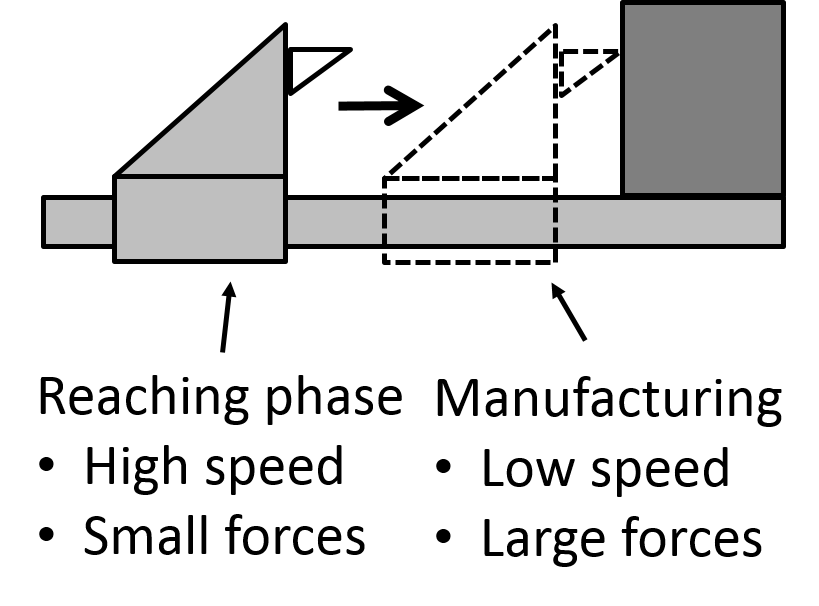
\includegraphics[width=0.25\textwidth]{machinetool.png}
				\label{fig:machinetool}}
        \subfloat[Legged robot]{
				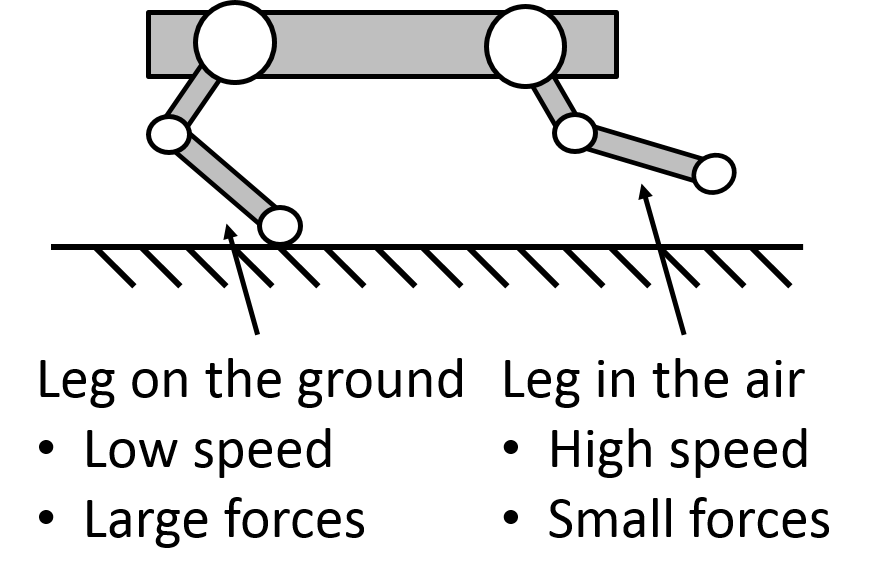
\includegraphics[width=0.25\textwidth]{leggedrobot.png}
				\label{fig:leggedrobot}}
				\subfloat[Gripper]{
				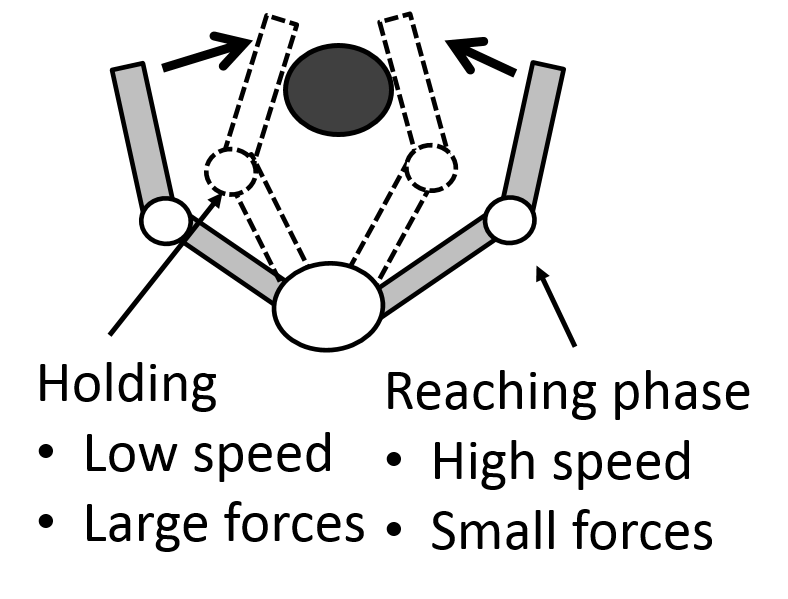
\includegraphics[width=0.25\textwidth]{gripper.png}
				\label{fig:gripper}}
        \caption{Robotics system encountering very different load situation}
				\label{fig:app}
\end{figure}


\section{Proposed solution: Robots using multiple gear-ratio actuators}
\label{sec:ProposedSolutionRobotsUsingMultipleGearRatioActuators}


\begin{figure}[H]
	\centering
		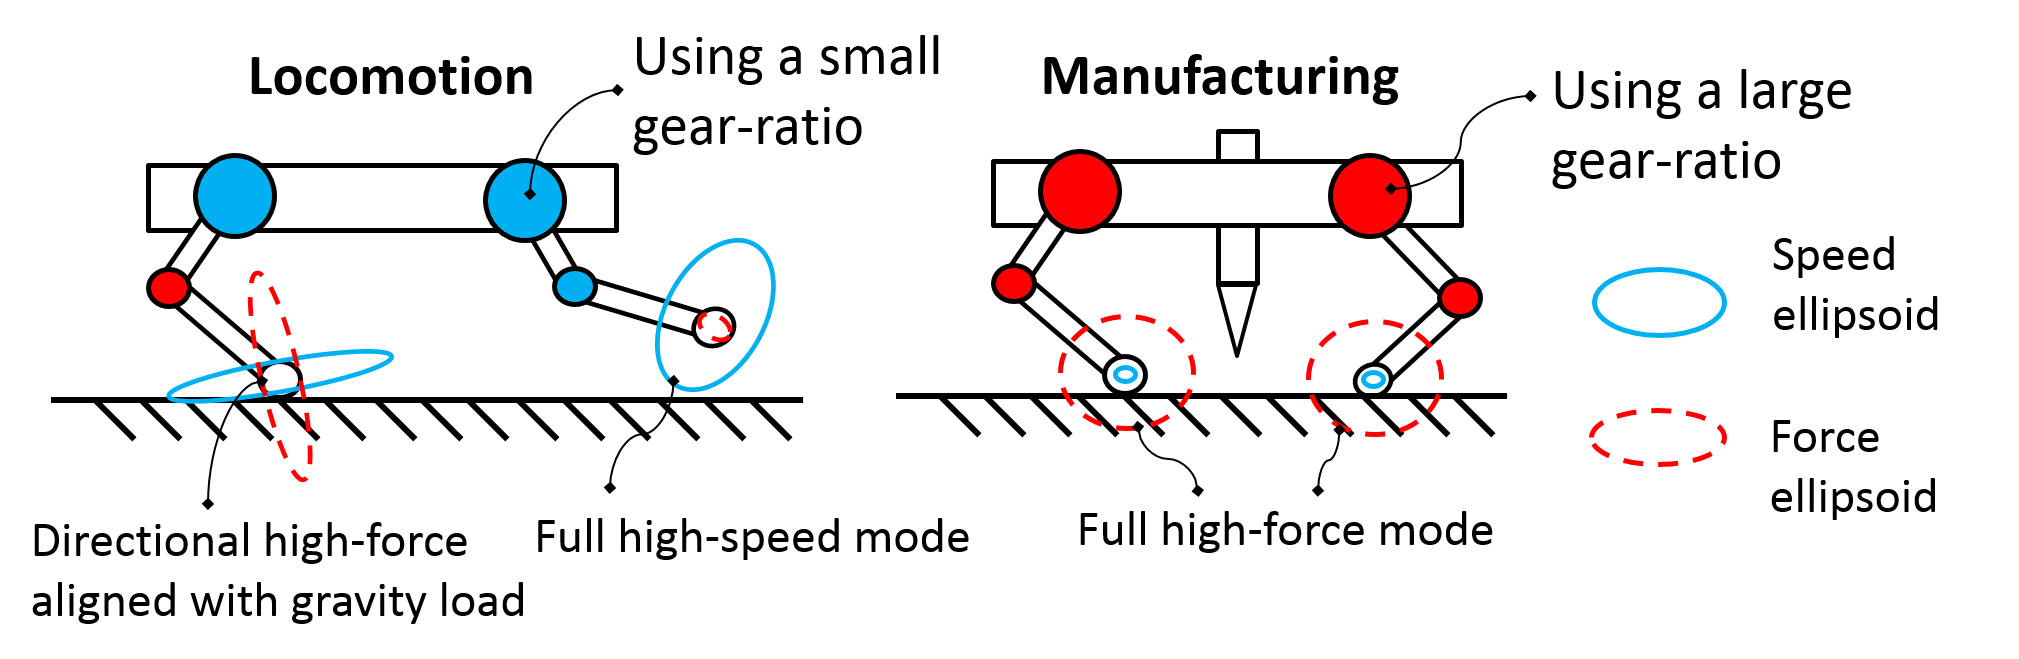
\includegraphics[width=0.90\textwidth]{gearselectionlegged.png}
	\caption{Example of advantageous gear selection with a multi-DOF robot}
	\label{fig:gearselectionlegged}
\end{figure}


\section{Main challenges}
\label{sec:MainChallenges}

\subsection{Actuator design}
\label{sec:ActuatorDesign}

\subsection{Control and planning of hybrid system}
\label{sec:ControlAndPlanningOfHybridSystem}



\section{Original contributions}
\label{sec:contribution}


\section{Organization of the thesis}
\label{sec:OrganisationOfTheThesis}




